\chapter{\babTiga}

\section{Tahapan Penelitian}

Pada penelitian ini akan dilakukan dalam beberapa tahapan. Tahap yang pertama
adalah studi literatur untuk mempelajari dan memahami materi-materi terkait
dengan penelitian, seperti \tracking~serta arsitektur \pubsub. Tahapan yang
kedua yaitu melakukan analisa. Tahap ketiga adalah mengimplementasikan hasil
analisa. Selanjutnya, tahap keempat yaitu melakukan ujicoba hasil implementasi
pada lingkungan ujicoba yang telah disiapkan. Dan tahap yang terakhir adalah
melakukan evaluasi hasil dari uji coba dan membuat laporan akhir. Skema tahapan
penelitian dapat dilihat pada Gambar~\ref{fig:tahapan}. Tahapan-tahapan ini
akan dikerjakan sesuai dengan jadwal yang terlampir pada Tabel~\ref{tab:jadwal}
pada halaman~\pageref{tab:jadwal}. 

\begin{figure}
    \centering
    \begin{tikzpicture}[font=\footnotesize, node distance=2em, auto]
        \node[cloud] (mulai) {Mulai};
        \node[block, right=1em of mulai] (literatur) {Studi literatur};
        \node[block, right=1em of literatur] (analisa) {Analisis dan desain};
        \node[block, right=1em of analisa] (implementasi) {Implementasi};
        \node[block, below of=analisa] (ujicoba) {Uji coba dan evaluasi};
        \node[block, below of=literatur] (laporan) {Penulisan laporan};
        \node[cloud, left=1em of laporan] (selesai) {Selesai};

        \path[arrow] (mulai) -- (literatur);
        \path[arrow] (literatur) -- (analisa);
        \path[arrow] (analisa) -- (implementasi);
        \path[arrow] (implementasi) |- (ujicoba);
        \path[arrow] (ujicoba) -- (laporan);
        \path[arrow] (laporan) -- (selesai);
    \end{tikzpicture}
    \caption{Diagram Alir Tahapan Penelitian}
\label{fig:tahapan}
\end{figure}
\begin{enumerate}[noitemsep,nolistsep,leftmargin=0cm,itemindent=.5cm,listparindent=\parindent]
    \item Studi Literatur

Dalam studi literatur, dikaji berbagai referensi mengenai konsep \tracking~dan
arsitektur \pubsub~serta karakteristik \context~\aware. Dari hasil studi
literatur ini, dapat ditemukan kekurangan dan kelebihan dari masing-masing
topik. \Tracking~yang efisien harus bersifat adaptif dan efisien dalam energi
karena proses pembaharuan yang bersifat sekuensial. Pada sistem
\pubsub~mempunyai kelebihan yang dapat diadopsi pada proses \tracking, terutama
dalam proses \tracking~multi target.

    \item Analisis dan Desain

Tahap awal analisis dan desain adalah merumuskan kontribusi utama penelitian
ini.  Dari studi literatur yang telah dilakukan, dapat diketahui bahwa sistem
\tracking~memerlukan mekanisme yang efisien dalam energi dan pembaharuan.
Sistem \tracking~adaptif terhadap kebutuhan tingkat presisi suatu lokasi.
Dalam tahap desain, dijelaskan langkah-langkah dalam proses pengerjaan
penelitian.  Rancangan telah dibagi dalam modul-modul sehingga akan mempermudah
dalam tahap implementasi.

\item Implementasi

Dalam tahap ini, diimplementasikan rancangan yang telah dibuat pada proses
sebelumnya.  Bahasa pemrograman yang digunakan adalah bahasa Java pada sisi
client maupun server.  Implementasi dilakukan pada \f{smartphone} bersistem
operasi android pada sisi klien, dan pada sisi server dikembangan dengan
bantuan ActiveMQ sebagai sistem \pubsub. ActiveMQ mendukung protokol MQTT (MQ
Telemetry Transport), sebuah protokol yang ringan dalam sistem \pubsub~sehingga
cocok digunakan dalam komunikasi pada jaringan bergerak.

\item Uji Coba dan Evaluasi

Untuk menguji apakah kontribusi yang diajukan dapat berjalan dengan baik, perlu
dilakukan uji coba. Uji coba dilakukan pada \f{smartphone} dalam suatu area
yang telah ditentukan dengan berbagai kondisi. Skenario uji coba dilakukan
dengan memberikan berbagai beban kerja pada proses \tracking. Hasil uji coba
akan dievaluasi dan dapat dilihat kinerja metode yang diajukan.

\item Penulisan Laporan Penelitian

Tahap ini adalah tahap untuk menyusun laporan penelitian. Setiap kegiatan yang
dilakukan dalam penelitian akan didokumentasikan. Laporan berisi penjelasan
mulai dari tahap studi literatur, analisa, tahap ujicoba serta kesimpulan dan
saran.  Laporan penelitian ditulis sesuai dengan ketentuan yang berlaku.

\end{enumerate}
\section{Langkah-langkah Penelitian}

Langkah-Langkah penelitian secara umum disajikan dalam
Gambar~\ref{fig:langkah}.  Langkah pertama adalah mempersiapkan lingkungan
\pubsub, yaitu instalasi \f{ActiveMQ}.  Selanjutnya, mempersiapkan data sampel
yang digunakan dalam \f{activity recognition}.  Langkah selanjutnya adalah
mengimplementasikan \tracking~multi target, implementasi dilakukan pada sisi
\client~serta~\server. Kemudian, dilakukan uji coba dan evaluasi untuk
mengetahui kinerja dari metode yang diajukan pada lingkungan uji coba yang
telah disiapkan dalam penelitian ini.

Dalam mempersiapkan lingkungan \pubsub~diperlukan suatu \f{middleware}, yaitu
\activemq. \f{Middleware} ini dibangun menggunakan bahasa pemrograman Java.
Oleh karena itu sebelum konfigurasi \activemq~dilakukan, diperlukan pengaturan
lingkungan JAVA\_HOME pada sistem operasi. Sistem operasi yang dipilih adalah
Linux, dikarenakan kemudahan dalam konfigurasi serta kehandalannya. Banyak 
metode dalam mengatur konfigurasi \activemq, tetapi dalam penelitian ini akan
dilakukan dengan konfigurasi berkas XML sebagai parameter.

%\tikzstyle{decision} = [diamond, draw, aspect=2, 
    %text width=4em, text badly centered, node distance=3cm, inner sep=0pt]
%\tikzstyle{block} = [rectangle, draw, node distance=2cm, 
    %text width=10em, text centered, minimum height=2em]
%\tikzstyle{line} = [draw, -latex]
%\tikzstyle{cloud} = [draw, ellipse, node distance=2cm, 
    %minimum height=2em]

\begin{figure}
    \centering
    \begin{tikzpicture}[font=\small, node distance=2cm, auto]
        \node[cloud] (start) {Mulai};
        \node[block, below of=start] (a) {Mempersiapkan lingkungan \pubsub};
        \node[block, below of=a] (b) {Mempersiapkan data sampel};
        \node[block, below of=b] (c) {Implementasi \tracking~multi target};
        \node[block, below of=c] (d) {Mempersiapkan lingkungan uji coba};
        \node[block, below of=d] (e) {Uji coba dan evaluasi};
        \node[cloud, below of=e] (end) {Selesai};

        \path[arrow] (start) -- (a);
        \path[arrow] (a) -- (b); 
        \path[arrow] (b) -- (c); 
        \path[arrow] (c) -- (d); 
        \path[arrow] (d) -- (e);
        \path[arrow] (e) -- (end); 
    \end{tikzpicture}
    \caption{Langkah-langkah penelitian secara umum}
\label{fig:langkah}
\end{figure}

%\begin{figure}
    %\centering
    %\begin{tikzpicture}[font=\small, node distance=2cm, auto]
        %\node[cloud] (start) {Mulai};
        %\node[block, below of=start] (a) {Instalasi sistem operasi Linux};
        %\node[block, below of=a] (b) {Instalasi Java (JDK)};
        %\node[block, below of=b] (c) {Instalasi dan konfigurasi \activemq};
        %\node[cloud, below of=c] (end) {Selesai};

        %\path[line] (start) -- (a);
        %\path[line] (a) -- (b); 
        %\path[line] (b) -- (c); 
        %\path[line] (c) -- (end); 
    %\end{tikzpicture}
    %\caption{Langkah-langkah mempersiapkan lingkungan \pubsub}
    %\label{fig:lingkungan_pubsub}
%\end{figure}

\section{Rancangan Sistem}

Pada penelitian sebelumnya (Kjaergaard dkk, 2009) telah diimplementasikan
sistem \tracking~yang efisien untuk perangkat bergerak. Sayangnya sistem
\tracking~ini kurang mengakomodir untuk proses \tracking~multi target. Sistem
\pubsub~ideal pada lingkungan jaringan tak handal seperti WSN (Hunkeler dkk,
2008). Karena karakter lingkungan WSN yang hampir sama dengan jaringan
bergerak, hal ini dapat diadopsi. 

Interaksi antara \publisher~(entitas yang menjadi target \tracking) dengan
\subscriber~(entitas yang melakukan \tracking~atau \f{tracker}) dapat dipaparkan pada
Gambar~\ref{fig:sistem}.  \Publisher~akan mengirimkan \event~kepada sistem
\pubsub~berupa informasi \tracking.  Sedangkan \subscriber~mengirimkan
\subscription~yang diatur dalam \f{subscription language} kepada sistem
\pubsub, \subscriber~hanya akan dinotifikasi sesuai dengan ketertarikannya
melalui proses \f{content-filtering}. Notifikasi ke entitas \subscriber, akan
ditangani oleh \f{event notification}. Entitas \subscriber~dapat berwujud
\f{mobile client} maupung \f{web client}. Sistem \pubsub~mengatur masa
\subscription~entitas \subscriber, jika telah melewati masa kadaluarsa maka
\publisher~akan dinotifikasi untuk menghentikan proses \publish.

Dalam perangkat bergerak, ditanamkan sebuah modul adaptif dalam penentuan
lokasi.  Modul ini akan mendeteksi aktifitas obyek yang diamati, dari aktifitas
ini menjadi dasar klasifikasi kebutuhan pembaruan serta presisi lokasi. Deteksi
aktifitas didasarkan pada data \f{sampling} yang direkam menggunakan sensor
\acc.


\noindent
\begin{figure}
    \centering
    \begin{tikzpicture}[font=\small, node distance=2cm, auto]
        \node[cloud] (start) {Mulai};
        \node[decision, below of=start] (a) {Deteksi mode \tracking?};
        \node[block, below of=a] (b) {\Tracking};
        \node[block, below of=b] (c) {Penjadwalan untuk pengecekan status};
        
        \coordinate(A) at ($ (a) + (-4, 0) $);
        \coordinate(B) at ($ (a) + (4, 0) $);

        \path[line] (start) -- (a);
        \path[line] (a) -- node [near start] {Ya} (b);
        \path[line] (a) -- (B) |- node [near start] {Tidak} (c); 
        \path[line] (b) -- (c); 
        \path[line] (c) -| (A) -- (a);
        
    \end{tikzpicture}
    \caption{Diagram alir sistem \tracking}
\label{fig:tracking}
\end{figure}

Interaksi pada sistem \pubsub~tradisional, walaupun informasi dari \publisher~tidak
dibutuhkan, pihak \publisher~akan tetap mem-\publish~informasi ke server. Untuk
mengurangi hal ini, diperlukan mekanisme untuk menangani masalah ini seperti
terlampir pada Gambar~\ref{fig:tracking}. Sedangkan untuk proses \tracking~akan
mengadopsi diagram dari sistem EnTracked seperti yang tertera pada
Gambar~\ref{fig:movement}. Dalam komunikasi data pada proses \tracking~akan
digantikan dengan skema \pubsub~dengan protokol MQTT (MQ Telemetry Transport).

\noindent
\begin{figure}
    \centering
    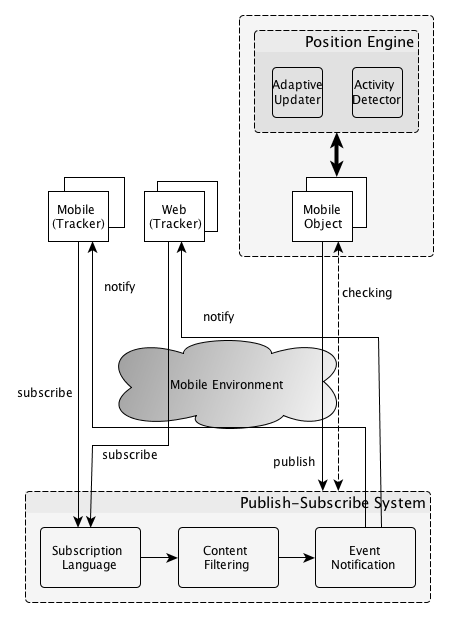
\includegraphics[scale=0.80]
        {pics/sistem.png}
    \caption{Arsitektur rancangan sistem}
\label{fig:sistem}
\end{figure}

%\tikzstyle{decision} = [diamond, draw, aspect=2, 
    %text width=4em, text badly centered, node distance=3cm, inner sep=0pt]
%\tikzstyle{block} = [rectangle, draw, node distance=3cm, 
    %text width=10em, text centered, minimum height=2em]
%\tikzstyle{line} = [draw, -latex]
%\tikzstyle{dash} = [draw, -latex, dashed] 
%\tikzstyle{doublearrow} = [draw, latex'-latex', double]
%\tikzstyle{cloud} = [draw, ellipse, node distance=2cm, 
%    minimum height=2em]
%\begin{figure}
    %\centering
    %\begin{tikzpicture}[font=\small, node distance=2cm, auto]
        %\node[block] (pubsub) {Sistem \PubSub};
        %\node[cloud, below=4cm of pubsub] (ta) {T1};
        %\node[cloud, right of=ta] (tb) {T2};
        %\node[cloud, right of=tb] (tc) {T3};
        %\node[cloud, left of=ta] (ua) {U1};
        %\node[cloud, left of=ua] (ub) {U2};
        %\node[cloud, left of=ub] (uc) {U3};

        %\path[line] (ta) -- (pubsub);
        %\path[line] (tb) -- (pubsub);
        %\path[line] (tc) -- (pubsub);

        %\path[line] (ua) -- (pubsub);
        %\path[line] (ub) -- (pubsub);
        %\path[line] (uc) -- (pubsub);

        %\path[dash] (pubsub) -- ([xshift=5pt] ta.north);
        %\path[dash] (pubsub) -- ([xshift=5pt] tb.north);
        %\path[dash] (pubsub) -- ([xshift=5pt] tc.north);
       
        %\path[dash] (pubsub) -- ([xshift=-5pt] ua.north);
        %\path[dash] (pubsub) -- ([xshift=-5pt] ub.north);
        %\path[dash] (pubsub) -- ([xshift=-5pt] uc.north);

        %\node at ($ (pubsub) + (0, 1) $) {\f{Content-filtering}}; 
    %\end{tikzpicture}
    %\caption{Rancangan sistem secara umum}
    %\label{fig:sistem}
%\end{figure}
\section{Location Model}
\label{sec:location_model}

Pada proses komunikasi antara \f{tracker} dengan obyek yang menjadi target
\tracking~terjadi pertukaran data. Dengan ini diperlukan pemodelan data yang
dikirimkan. Dalam Tabel~\ref{tab:model} dipaparkan pemodelan data yang dimaksud.
Setiap target \tracking~mempunyai atribut ID, Name, Role, Lat, Long dan Time.
Deskripsi setiap atribut dijelaskan pada kolom Keterangan. 

\begin{table}
\centering
\caption{Data Model}
\label{tab:model}
\begin{tabular}{l l l}
        \hline
        Atribut & Tipe & Keterangan \\
        \hline
        ID      & String    & Informasi identitas obyek yang di-\f{track} \\
        Name    & String    & Nama dari obyek yang di-\f{track} \\
        Role    & String    & Informasi hak akses dari obyek yang di-\f{track} \\
        Lat     & Float     & Nilai \f{latitude} \\
        Long    & Float     & Nilai \f{longitude} \\
        Time    & Date Time & Informasi mengenai waktu data dikirimkan \\
        \hline
    \end{tabular}
\end{table}

Dalam pemodelan data terdapat atribut Role, yang berfungsi untuk membedakan
level hak akses seperti yang dipaparkan pada Tabel~\ref{tab:level}. Atribut
Role dibagi menjadi tiga level hak akses, yaitu: Role 1, Role 2 dan Role 3.
Pembedaan level ini mempengaruhi tingkat resolusi spasial yang berkaitan dengan
privasi target \tracking. Semakin tinggi level suatu \Role, mempunyai hak akses
yang lebih luas, contoh: Role 1 mempunyai resolusi spasial sampai level 3, sedangkan
Role 3 hanya mempunyai sampai level 1.

\begin{table}
\centering
\caption{Level Hak Akses}
\label{tab:level}
\begin{tabular}{l l}
   \hline
   Role     & Hak Akses     \\
   \hline
   Role 1   & Level 1~-~Level 3 \\
   Role 2   & Level 1~-~Level 2 \\
   Role 3   & Level 1 \\
   \hline
\end{tabular}
\end{table}

Pemodelan lokasi yang digunakan merupakan gabungan antara \f{Geometric} dan
\f{Symbolic} yang bersifat hirarkis. Resolusi suatu informasi lokasi
dipengaruhi oleh level hak akses, \tracker~yang mempunyai \Role~lebih tinggi
atau selevel dengan target \tracking~memiliki resolusi informasi yang lebih
detil.  Pada Gambar~\ref{fig:skema} lingkungan Kampus Institut Teknologi
Sepuluh Nopember (ITS) dibagi menjadi tiga tingkat level. Seorang \tracker~yang
mempunyai hak akses level 1 hanya dapat mengetahui informasi sebatas target
\tracking~sedang berada di wilayah kampus ITS atau tidak. Sedangkan untuk
\tracker~yang mempunyai hak akses lebih tinggi dapat memperoleh informasi
sampai level gedung/bangunan.

\begin{figure}
\centering
    \begin{tikzpicture}[font=\small, node distance=2cm, auto]
        \node[cloud] (map) {Peta};
        \coordinate(A) at ($ (map) + (0,-2) $);
        \node[cloud, left=2cm of A] (outits) {Luar ITS};
        \node[cloud, right=2cm of A] (its) {Kampus ITS};
        \coordinate(L10) at ($ (outits) + (0,1) $);
        \coordinate(L11) at ($ (its) + (0,1) $);
        \node at ($ (L11) + (1,0) $) {Level 1};

        \coordinate(B) at ($ (its) + (0,-2) $);
        \node[cloud, left=2cm of B] (area1) {Area 1};
        \node[cloud, right=2cm of B] (area2) {Area 2};
        \coordinate(L20) at ($ (area1) + (0,1) $);
        \coordinate(L21) at ($ (area2) + (0,1) $);
        \node at ($ (L20) + (-1,0) $) {Level 2};

        \coordinate(C) at ($ (area1) + (0,-2) $);
        \node[cloud, left=2cm of C] (jurusan1) {Jurusan 1};
        \node[cloud, right=2cm of C] (jurusan2) {Jurusan 2};
        \coordinate(L30) at ($ (jurusan1) + (0,1) $);
        \coordinate(L31) at ($ (jurusan2) + (0,1) $);
        \node at ($ (L31) + (1,0) $) {Level 3};

        \path[arrow] (map) -- (outits);
        \path[arrow] (map) -- (its);
        \path[arrow] (its) -- (area1);
        \path[arrow] (its) -- (area2);
        \path[arrow] (area1) -- (jurusan1);
        \path[arrow] (area1) -- (jurusan2);

        \path[line,dashed] (L10) -- (L11);
        \path[line,dashed] (L20) -- (L21);
        \path[line,dashed] (L30) -- (L31);
    \end{tikzpicture}
\caption{\LocationModel}
\label{fig:skema}
\end{figure}

\section{\f{Sampling} Deteksi Aktifitas}

\noindent
\begin{figure}
\centering
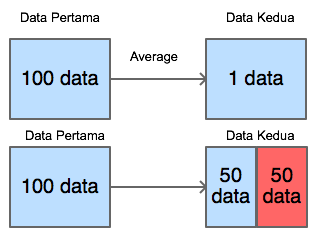
\includegraphics[scale=1]
    {pics/sampling.png}
    \caption{\f{Windows Sampling} dan \f{Overlapping}}
\label{fig:windows-sampling}
\end{figure}

Dalam proses \f{activity recognition} diperlukan data sampel. Keakuratan sebuah data
merupakan hal yang sangat penting sebagai langkah awal dalam klasifikasi. Agar
kebutuhan tersebut terpenuhi maka diperlukan suatu teknik interpretasi data
yang khusus. Salah satu cara mengektraksi data dengan \f{windows sampling},
yaitu suatu teknik mengektraksi data dengan \f{sampling} data, setiap
\f{windows} terdiri dari kumpulan data yang akan merepresentasikan satu buah
data.

Cara pengambilan \f{sampling} data dapat dipaparkan pada
Gambar~\ref{fig:windows-sampling}. Dalam
pengambilan data X dengan menggunakan sensor Y, misalnya setiap satu detik
sensor Y menghasilkan seratus perubahan data. 100 data tersebut dapat
direpresentasikan dalam satu data menggunakan nilai rata-rata yang ditunjukkan
pada Gambar~\ref{fig:windows-sampling}. \f{Overlapping} digunakan untuk menjaga
agar data tetap konsisten sehingga data tidak terlalu divergen. Untuk
pengambilan data berikutnya (kedua dan seterusnya), setengah dari \f{windows}
diambil dari data sebelumnya dan setengah lagi dari perubahan sensor berikutnya.

%\begin{figure}
    %\centering
    %\begin{tikzpicture}[font=\small, node distance=2cm, auto]
        %\node[block] (a) {\bo{100 data}};
        %\node[block, right=3cm of a] (b) {\bo{1 data}};
        
        %\node at ($ (a) + (0, 1) $) {\f{Windows Sampling}};
        %\path[line] (a) -- node [near start] {Average} (b);
    %\end{tikzpicture}
    %\caption{Teknik \f{windows sampling}}
    %\label{fig:windows}
%\end{figure}

%\begin{figure}
    %\centering
    %\begin{tikzpicture}[font=\small, node distance=2cm, auto]
        %\node[block] (a) {\color{blue}{\bo{100 data}}};
        %\node[block, right=3cm of a] (b) 
            %{\color{blue}{\bo{50 data}} $\vert$ \color{black}$\vert$ {\bo{50 data}}};

        %\node at($ (a) + (0, 1) $) {Data pertama};
        %\node at($ (b) + (0, 1) $) {Data kedua};

        %\path[line] (a) -- (b);
    %\end{tikzpicture}
    %\caption{Teknik \f{overlapping}}
    %\label{fig:overlapping}
%\end{figure}

\section{Uji Coba dan Evaluasi}

Pada bagian ini dipaparkan mengenai lingkungan yang dijadikan uji coba dan
evaluasi. Pada sistem \tracking~multi target ini terdapat dua komponen utama,
yaitu client dan server.  Client merupakan entitas yang menjadi target
\tracking~atau yang melakukan \tracking. Client yang menjadi target
\tracking~berupa perangkat \f{smartphone}, sedangkan pelaku \tracking~dapat
berupa \f{smartphone} maupun web. Pada sisi server terdapat sebuah sistem
\pubsub~tunggal, yang memiliki \f{IP public}. Sistem \pubsub~dibangun
menggunakan \activemq, dan untuk protokol komunikasi dengan client menggunakan
protokol MQTT.

\begin{figure}
    \centering
    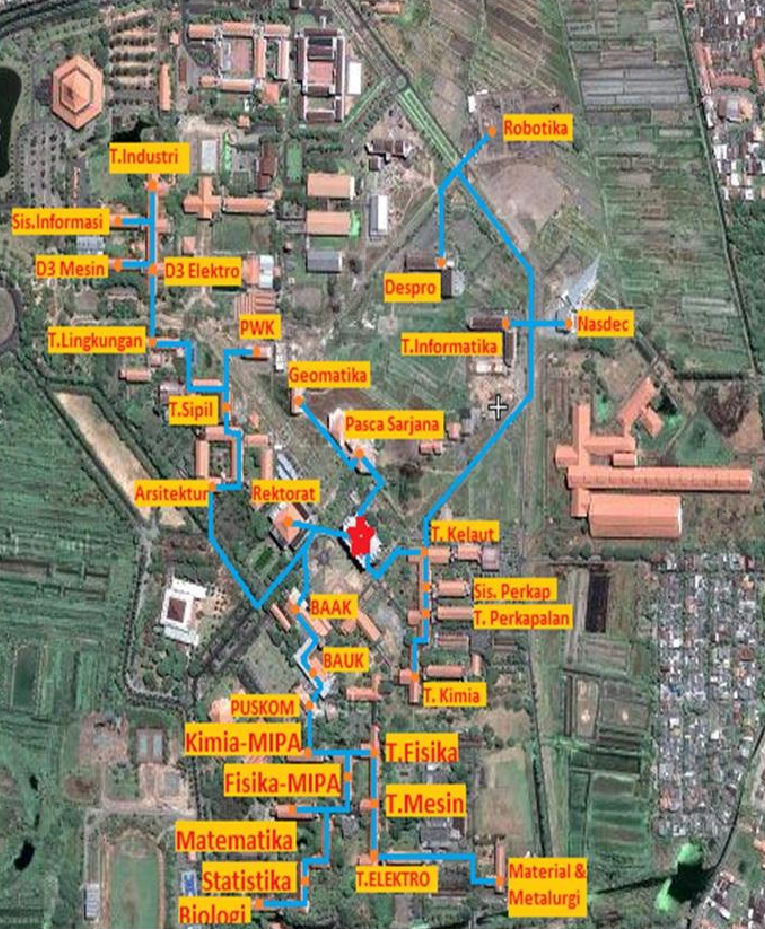
\includegraphics[scale=0.32]
        {pics/its.png}
    \caption{Denah lokasi kampus Institut Teknologi Sepuluh Nopember}
\label{fig:its}
\end{figure}

Area \tracking~yang digunakan adalah area kampus Insitut Teknologi
Sepuluh Nopember (Gambar~\ref{fig:its}) yang sudah dilakukan pemodelan lokasi. 
Pembatasan area ini untuk memudahkan pengujian dan analisa. Proses
\tracking~dilakukan pada orang yang bergerak dengan berjalan kaki (pedestrian)
tanpa bantuan kendaraan. 

Uji coba dilakukan dengan menghitung banyaknya paket yang dikirimkan, serta
banyaknya pengurangan paket setelah modul adaptif diaktifkan dengan parameter
yang berbeda pada lingkungan uji coba yang telah disiapkan.  Parameter itu
berupa jumlah target \tracking, jarak interval pembaruan lokasi dengan variasi
jumlah \publisher~dengan \subscriber. Jumlah \publisher~dan \subscriber~yang direncanakan
dalam pengujian adalah 10. Dari perhitungan ini, didapatkan seberapa
signifikan efisiensi sistem \tracking~multi target.

\section{Jadwal Kegiatan Penelitian}

Pada Tabel~\ref{tab:jadwal} diuraikan mengenai jadwal kegiatan penelitian
selama empat bulan. Jadwal akan dipetakan perminggu dalam empat bulan pengerjaan.

\begin{table}
\centering
\caption{Jadwal Kegiatan}
\label{tab:jadwal}
    \begin{tabular}{|p{50mm}|p{1mm}|p{1mm}|p{1mm}|p{1mm}|p{1mm}|p{1mm}|p{1mm}|p{1mm}|p{1mm}|p{1mm}|p{1mm}|p{1mm}|p{1mm}|p{1mm}|p{1mm}|p{1mm}|}
        \hline
        \multicolumn{1}{|c|}{\multirow{2}{*}{Kegiatan}} & \multicolumn{4}{|c|}{\bulanSatu} & \multicolumn{4}{|c|}{\bulanDua} & \multicolumn{4}{|c|}{\bulanTiga} & \multicolumn{4}{|c|}{\bulanEmpat} \\
        & \multicolumn{4}{|c|}{\tahun} & \multicolumn{4}{|c|}{\tahun} & \multicolumn{4}{|c|}{\tahun} & \multicolumn{4}{|c|}{\tahun} \\ \hline 
        Studi Literatur     &\g &\g &\g &\g     & ~ & ~ & ~ & ~     & ~ & ~ & ~ & ~     & ~ & ~ & ~ & ~ \\ \hline
        Analisa dan desain  & ~ & ~ & ~ & ~     &\g &\g &\g & ~     & ~ & ~ & ~ & ~     & ~ & ~ & ~ & ~ \\ \hline
        Implementasi        & ~ & ~ & ~ & ~     & ~ & ~ &\g &\g     &\g &\g &\g &\g     &\g & ~ & ~ & ~ \\ \hline
        Uji coba            & ~ & ~ & ~ & ~     & ~ & ~ & ~ & ~     & ~ & ~ & ~ & ~     & ~ &\g &\g &\g \\ \hline
        Penulisan Laporan   & ~ &\g &\g &\g     &\g &\g &\g &\g     &\g &\g &\g &\g     &\g &\g &\g &\g \\
        \hline
    \end{tabular}
\end{table}
